
\begin{figure}[h]
    \centering
    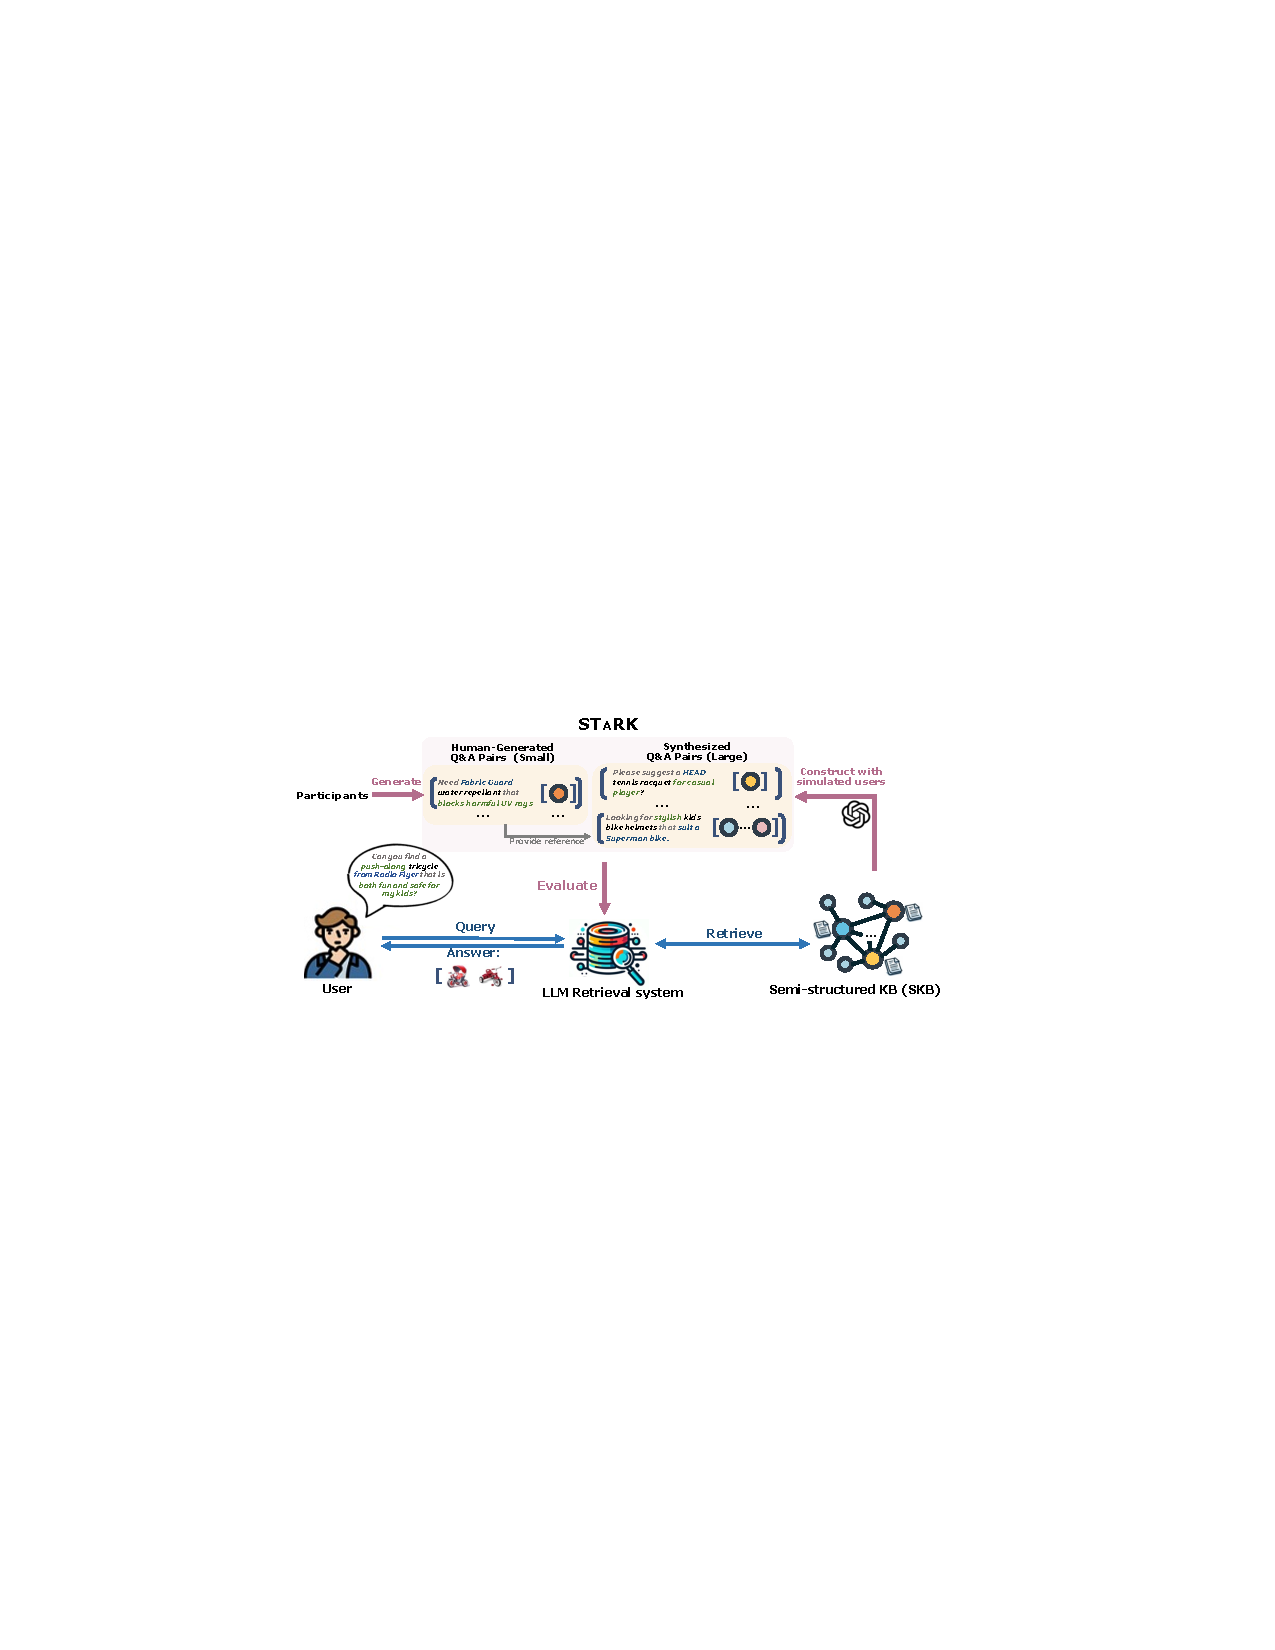
\includegraphics[width=0.90\textwidth]{figs/overview2}
    \caption{
    % Overview of the task and benchmark: 
    % Benchmarking retrieval systems on semi-structure knowledge bases with textual and relational information. 
    % \michi{Please provide more detailed caption to explain this figure. Whether Figure 1 is easy to understand or not is crucial, really influences readers' impression of this paper.}\kexin{i feel like it is hard to know where to start reading this figure. maybe add more annotations? for example, the upper part of figure can be shaded box and annotate with STAR benchmark and bottom part is the use case.}
    \benchmarkh features queries on Semi-structured Knowledge Base (SKB) with textual and relational knowledge, with node entities as ground-truth answers. \revision{\benchmarkh consists of synthesized queries simulating user interactions with a SKB and human-generated queries which provide an authentic reference. }It evaluates LLM retrieval systems' performance in providing accurate responses. 
    }
    \label{fig:task}
\end{figure}


% \begin{table}<t>
%     \resizebox{1.0\textwidth}{!}{
%     \begin{tabular}{ccc}
%         \toprule
%         & {Target} & {Example query} \\
%         \midrule
%         \hline
%         \multirow{4}{*}{\amazont} & \multirow{ 4}{*}{\texttt{product}} & \cellcolor{cyan!5} {\textit{Looking for \textcolor{OliveGreen}{durable} \textcolor{MidnightBlue}{Dart World brand} {dart flights} that}}\\
%          & & \cellcolor{cyan!5} {\textit{\textcolor{OliveGreen}{resist easy tearing}. Any recommendations?}}  \\
%         % \cellcolor{cyan!5} {\textit{Can you help me find a \textcolor{OliveGreen}{push-along} tricycle \textcolor{MidnightBlue}{from Radio Flyer} that's  }}  \\
%         % & & \cellcolor{cyan!5} {\textit{\textcolor{OliveGreen}{both fun and safe for my kid}?}}  \\
%         \noalign{\vspace{0.75ex}}
%         &&\cellcolor{cyan!5} {\textit{What are recommended {scuba diving weights} \textcolor{OliveGreen}{for experienced divers} }}\\
%         &&\cellcolor{cyan!5} {\textit{that would \textcolor{MidnightBlue}{fit well with my Gorilla PRO XL waterproof bag}?}}\\
%         \noalign{\vspace{0.7ex}}
%         \midrule
%         \noalign{\vspace{0.7ex}}
%         \multirow{ 3}{*}{\magt} & \multirow{ 3}{*}{\texttt{paper}} & \cellcolor{yellow!10} {\textit{Search {publications} \textcolor{MidnightBlue}{by Hao-Sheng Zeng} on \textcolor{OliveGreen}{non-Markovian dynamics}.}} \\
%         \noalign{\vspace{0.75ex}}
%         & &  \cellcolor{yellow!10}\textit{What are some \textcolor{OliveGreen}{nanofluid heat transfer} {research papers} published by}\\
%         & &  \cellcolor{yellow!10}\textit{scholars \textcolor{MidnightBlue}{from Philadelphia University}?} \cellcolor{yellow!10}\\
%         \noalign{\vspace{0.7ex}}
%         \midrule
%         \noalign{\vspace{0.75ex}}
%         \multirow{6}{*}{\primekgt} & \multirow{ 2}{*}{\texttt{drug}} &  \cellcolor{pink!20}\textit{Could you provide a list of \textcolor{OliveGreen}{investigational} {drugs} that }\\
%         && \cellcolor{pink!20}\textit{\textcolor{MidnightBlue}{interact with genes or proteins active in the epididymal region}?}\\
%         \noalign{\vspace{0.7ex}}
%         % & \multirow{ 1}{*}{\texttt{disease}}
%         % & \cellcolor{pink!20}\textit{Is my \textcolor{OliveGreen}{constant fatigue} due to conditions \textcolor{MidnightBlue}{related to bartonellosis}?}\\
%         & \multirow{ 2}{*}{\texttt{disease}}
%         & \cellcolor{pink!20}\textit{Search for {diseases} \textcolor{MidnightBlue}{without known treatments} and induce}\\
%         && \cellcolor{pink!20}\textit{\textcolor{OliveGreen}{pruritus in pregnant women}, potentially \textcolor{MidnightBlue}{associated with Autoimmune}.}\\
%         \noalign{\vspace{0.75ex}}
%         & \texttt{pathway} & \cellcolor{pink!20}\textit{Please find {pathways} \textcolor{MidnightBlue}{involving the POLR3D gene} \textcolor{OliveGreen}{within nucleoplasm}.}\\
%         \noalign{\vspace{0.75ex}}
%         & \texttt{gene} & \cellcolor{pink!20}\textit{Which {gene} on \textcolor{OliveGreen}{chromosome 4} are \textcolor{MidnightBlue}{expressed in multicellular organisms}?}\\
%         \bottomrule
%     \end{tabular}
%     }
%     \vspace{2pt}
%     \caption{Example queries from \benchmarkt, where \textcolor{MidnightBlue}{relational} and \textcolor{OliveGreen}{textual} aspects are highlighted.}
%     \label{tab:benchmark_examples}
%     \vspace{-10pt}
% \end{table}


% \begin{table}<t>
%     \resizebox{1.0\textwidth}{!}{
%     \begin{tabular}{lcl}
%         \toprule
%         &{Example query} & {Answer(s):}  \texttt{node\_id}$_{<\texttt{name/title}>}$\\
%         \midrule
%         \hline
%         \multirow{4}{*}{\small \amazont}& \cellcolor{cyan!5} {\textit{Looking for \textcolor{OliveGreen}{durable} \textcolor{MidnightBlue}{Dart World brand} {dart flights} that}} & \cellcolor{cyan!5} {\texttt{1082} {\tiny{<Amazon Standard Flights>}}} \\
%          & \cellcolor{cyan!5} {\textit{\textcolor{OliveGreen}{resist easy tearing}. Any recommendations?}}  & \cellcolor{cyan!5} {{\texttt{236112}} {\tiny{<Dart World Broken Glass Flight> (12 more)}}}  \\
%         \noalign{\vspace{0.75ex}}
%         &\cellcolor{cyan!5} {\textit{What are recommended {scuba diving weights} \textcolor{OliveGreen}{for experienced divers} }} & \cellcolor{cyan!5} {\texttt{1725} {\tiny{<Sea Pearls Vinyl Coated Lace Thru Weight>}}}\\
%         &\cellcolor{cyan!5} {\textit{that would \textcolor{MidnightBlue}{fit well with my Gorilla PRO XL waterproof bag}?}}& \cellcolor{cyan!5} {}\\
%         \midrule
%         \multirow{ 4}{*}{\small \magt}  & \cellcolor{yellow!10} {\textit{Search {publications} \textcolor{MidnightBlue}{by Hao-Sheng Zeng} on \textcolor{OliveGreen}{non-Markovian dynamics}.}} & \cellcolor{yellow!10} {{\texttt{1565109}} {\tiny{<Distribution of non-Markovian intervals...>}}} \\
%         &\cellcolor{yellow!10}{} &\cellcolor{yellow!10} {{\texttt{1628038}} {\tiny{<Comparison between non-Markovian...>}}}\\
%         \noalign{\vspace{0.75ex}}
%         & \cellcolor{yellow!10}\textit{What are some \textcolor{OliveGreen}{nanofluid heat transfer} {research papers} published by} & \cellcolor{yellow!10} {\texttt{1564849} {\tiny{<A Numerical Study on Convection}}}\\
%         &  \cellcolor{yellow!10}\textit{scholars \textcolor{MidnightBlue}{from Philadelphia University}?}  & \cellcolor{yellow!10} {{\tiny{Around A Suqare Cylinder using AL2O3-H2O Nanofluid>}}}\\
%         \midrule
%         \multirow{6}{*}{\small  \primekgt} &  \cellcolor{pink!20}\textit{Could you provide a list of \textcolor{OliveGreen}{investigational} {drugs} that } & \cellcolor{pink!20}\texttt{19756} {\tiny{<(S)-3-phenyllactic Acid>}}\\
%         &\cellcolor{pink!20}\textit{\textcolor{MidnightBlue}{interact with genes or proteins active in the epididymal region}?} & \cellcolor{pink!20}\texttt{19882} {\tiny{<Anisomycin>}}, \texttt{19883} {\tiny{<Puromycin>}}\\
%         \noalign{\vspace{0.75ex}}
%         % & \multirow{ 1}{*}{\texttt{disease}}
%         % & \cellcolor{pink!20}\textit{Is my \textcolor{OliveGreen}{constant fatigue} due nto conditions \textcolor{MidnightBlue}{related to bartonellosis}?}\\
%         & \cellcolor{pink!20}\textit{Search for {diseases} \textcolor{MidnightBlue}{without known treatments} and induce} & \cellcolor{pink!20}\texttt{27746} {\tiny{<Intrahepatic Cholestasis>}}\\
%         &\cellcolor{pink!20}\textit{\textcolor{OliveGreen}{pruritus in pregnant women}, potentially \textcolor{MidnightBlue}{associated with Autoimmune}.} & \cellcolor{pink!20}\\
%         \noalign{\vspace{0.75ex}}
%         & \cellcolor{pink!20}\textit{Please find {pathways} \textcolor{MidnightBlue}{involving the POLR3D gene} \textcolor{OliveGreen}{within nucleoplasm}.}& \cellcolor{pink!20}{\small{\texttt{128961}}}{\tiny{<RNA Polymerase III Chain Elongation> (4 more)}} \\
%         \noalign{\vspace{0.75ex}}
%         & \cellcolor{pink!20}\textit{Which {gene} on \textcolor{OliveGreen}{chromosome 4} are \textcolor{MidnightBlue}{expressed in multicellular organisms}?} & \texttt{1151} {\tiny{<NFKB1>}}, \texttt{13501} {\tiny{<MT2P1>}}\cellcolor{pink!20}\\
%         \bottomrule
%     \end{tabular}
%     }
%     \vspace{2pt}
%     \caption{Example queries from \benchmarkt, where \textcolor{MidnightBlue}{relational} and \textcolor{OliveGreen}{textual} aspects are highlighted.}\small{
%     \label{tab:benchmark_examples}
%     \vspace{-10pt}
% \end{table}


\begin{table}
    \resizebox{1.00\textwidth}{!}{
    \begin{tabular}{lcl}
        \toprule
        &{Example query} & Title of ground-truth items(s) \\
        \midrule
        \hline
        \multirow{4}{*}{\amazont}& \cellcolor{cyan!5} {\textit{Looking for \textcolor{OliveGreen}{durable} \textcolor{MidnightBlue}{Dart World brand} {dart flights} that}} & \cellcolor{cyan!5}  {\small{<Amazon Standard Flights>}} \\
         & \cellcolor{cyan!5} {\textit{\textcolor{OliveGreen}{resist easy tearing}. Any recommendations?}}  & \cellcolor{cyan!5} {{\small{<Dart World Broken Glass Flight> (+12 more)}}}  \\
        \noalign{\vspace{0.75ex}}
        &\cellcolor{cyan!5} {\textit{What are recommended {scuba diving weights} \textcolor{OliveGreen}{for experienced divers} }} & \cellcolor{cyan!5} {{\small{<Sea Pearls Vinyl Coated Lace Thru Weight>}}}\\
        &\cellcolor{cyan!5} {\textit{that would \textcolor{MidnightBlue}{fit well with my Gorilla PRO XL waterproof bag}?}}& \cellcolor{cyan!5} {}\\
        \midrule
        \multirow{ 4}{*}{\magt}  & \cellcolor{yellow!10} {\textit{Search {publications} \textcolor{MidnightBlue}{by Hao-Sheng Zeng} on \textcolor{OliveGreen}{non-Markovian dynamics}.}} & \cellcolor{yellow!10} {{\small{<Distribution of non-Markovian intervals...>}}} \\
        &\cellcolor{yellow!10}{} &\cellcolor{yellow!10} {{\small{<Comparison between non-Markovian...>}}}\\
        \noalign{\vspace{0.75ex}}
        & \cellcolor{yellow!10}\textit{What are some \textcolor{OliveGreen}{nanofluid heat transfer} {research papers} published by} & \cellcolor{yellow!10} {{\small{<A Numerical Study on Convection Around A}}}\\
        &  \cellcolor{yellow!10}\textit{scholars \textcolor{MidnightBlue}{from Philadelphia University}?}  & \cellcolor{yellow!10} {{\small{Suqare Cylinder using AL2O3-H2O Nanofluid>}}}\\
        \midrule
        \multirow{6}{*}{\primekgt} &  \cellcolor{pink!20}\textit{Could you provide a list of \textcolor{OliveGreen}{investigational} {drugs} that } & \cellcolor{pink!20}{ \small{<(S)-3-phenyllactic Acid>}},\\
        &\cellcolor{pink!20}\textit{\textcolor{MidnightBlue}{interact with genes or proteins active in the epididymal region}?} & \cellcolor{pink!20}{ \small{<Anisomycin>}}, {\small{<Puromycin>}}\\
        \noalign{\vspace{0.75ex}}
        & \cellcolor{pink!20}\textit{Search for {diseases} \textcolor{MidnightBlue}{without known treatments} and induce} & \cellcolor{pink!20} {\small{<Intrahepatic Cholestasis>}}\\
        &\cellcolor{pink!20}\textit{\textcolor{OliveGreen}{pruritus in pregnant women}, potentially \textcolor{MidnightBlue}{associated with Autoimmune}.} & \cellcolor{pink!20}\\
        \noalign{\vspace{0.75ex}}
        & \cellcolor{pink!20}\textit{Please find {pathways} \textcolor{MidnightBlue}{involving the POLR3D gene} \textcolor{OliveGreen}{within nucleoplasm}.}& \cellcolor{pink!20}{\small{<RNA Polymerase III Chain Elongation>}} \\ %  (4 more)
        \noalign{\vspace{0.75ex}}
        & \cellcolor{pink!20}\textit{Which gene or protein \textcolor{MidnightBlue}{associated with lichen amyloidosis} can }& {\small{<OSMR>}},  {\small{<IL31RA>}}\cellcolor{pink!20}\\
        & \cellcolor{pink!20}\textit{\textcolor{OliveGreen}{bind interleukin-31 to activate the PI3K/AKT and MAPK pathways}?}& \cellcolor{pink!20}\\
        %& \cellcolor{pink!20}\textit{Which {gene} on \textcolor{OliveGreen}{chromosome 4} are \textcolor{MidnightBlue}{expressed in multicellular organisms}?} & {\small{<NFKB1>}},  {\small{<MT2P1>}}\cellcolor{pink!20}\\
        \bottomrule
    \end{tabular}
    }
    \vspace{2pt}
    \caption{\benchmarkh QA examples which involve semi-structured (\textcolor{MidnightBlue}{relational} and \textcolor{OliveGreen}{textual}) information. }
    \label{tab:benchmark_examples}
    \vspace{-15pt}
\end{table}

\section{Introduction}
\vspace{-6pt}
%%%%% INTRODUCE THE PROBLEM SETTING %%%%%
Natural-language queries are the primary form of how humans acquire information~\cite{hirschman2001natural, kaufmann2010evaluating,Jamil17}. 
% landscape of 
% \kexin{what is diverse landscape of knowledge? are you referring to diverse domains?}
For example, users on e-commerce sites wish to express complex information needs by combining free-form elements and constraints, such as ``\textit{Can you help me find a push-along tricycle from Radio Flyer that’s both fun and safe for my kid?}''\revision{ in product search. Medical scientists may ask questions like ``\textit{What disease is associated with the PNPLA8 gene and presents with hypotonia as a symptom?}''}.
% \jure{Add one more example from some other domain: science or medical}
Answering such queries is crucial for enhancing user experience, supporting informed decision-making, and preventing hallucination.

To answer such queries, the underlying knowledge can be represented in %semi-structured formats~\cite{UniK-QA,mag,RyuJK14}, referred to as 
semi-structured knowledge bases (SKBs)~\cite{UniK-QA,mag,RyuJK14}, which integrate unstructured data, such as natural language descriptions and expressions (\eg description of the tricycle), with structured data, like entity interactions on knowledge graphs
%\qian{I think using database is better, maybe database graph?} 
(\eg a tricycle ``brand'' is Radio Flyer). 
This allows the SKBs to represent comprehensive knowledge in specific applications, making them indispensable in domains such as e-commerce~\cite{ups-amazon_review}, social media~\cite{MansmannRWS14}, and precision medicine~\cite{primekg, ogb, Johnson2021}.

%%%% THE PROBLEM WE WANT TO SOLVE %%%%%%
%%%% + Why IS THIS IMPORTANT %%%%%%
%In this context, as shown in Figure~\ref{fig:task}, information retrieval serves as a predominant step by identifying relevant data from the SKBs, such as specific tricycles that match the request, which are then processed to generate accurate answers to user queries~\cite{Singhal01}.
%The retrieval accuracy on SKBs is crucial for enhancing user experience, supporting informed decision-making, and preventing hallucination.

%%%%%%%%%%% WHY HASN'T IT BEEN SOLVED %%%%%%%%
\xhdr{Limitations of prior works} Prior works focused on either purely textual queries on unstructured knowledge~\cite{IzacardG21, realm, KarpukhinOMLWEC20, LeeCT19, YangXLLTXLL19, dunn2017searchqa, TriviaQA, yang2018hotpotqa} or structured SQL~\cite{zhongSeq2SQL2017, yu-etal-2018-spider, zhongSeq2SQL2017, yu-etal-2018-spider} or knowledge graph queries~\cite{BerantCFL13, YihCHG15, h2t, ComplexWebQuestions, yih-etal-2016-value,talmor-berant-2018-web,cao-etal-2022-kqa,GAO_FODOR_KIFER_2019,he2024gretriever,AsaiHHSX20}, which are limited in the span of knowledge and inadequate to study the complexities of retrieval on SKBs. Recently, large language models (LLMs) have demonstrated significant potential on information retrieval tasks~\cite{llm4ir, realm, rag, replug}. Nevertheless, it remains an open question of how effectively LLMs can be applied to the challenging retrieval tasks on SKBs.  Moreover, the existing works mainly focus mainly on general knowledge, \eg from Wikipedia. However, the knowledge may commonly come from private sources, requiring retrieval systems to \revision{operate} on private SKBs. Therefore, there is a gap of how current LLM retrieval systems handle the complex textual and relational requirements in queries that can involve private knowledge. 

%%%%%%%%% WHY IS IT HARD %%%%%%%%%
% \kexin{i feel like here misses a transition sentence. Before here, you are discussing about this new problem setting of SKB and how previous works do not address them. In the next paragraph, you jump into talking about de details of building a benchmark for it. But you haven't motivated why do we need a benchmark for it and why is it hard to build this benchmark. }
\xhdr{Present work} 
To address this gap, we present a large-scale \underline{S}emi-structure retrieval benchmark on \underline{T}extual \underline{a}nd \underline{R}elational \underline{K}nowledge Bases (\benchmarkt) (Figure~\ref{fig:task}). The key technical challenge that we solve is how to accurately simulate user queries on SKBs. This difficulty arises from the interdependence of textual and relational information, which leads to challenges in precisely construct the ground-truth answers from millions of candidates. Additionally, ensuring that queries are useful and resembles real-world scenarios adds further complexity to the benchmarking process. 
 
We develop a novel pipeline that simulates user queries and constructs precise ground truth answers using three SKBs built from extensive texts and millions of entity relations from public sources.
We validate the quality of queries in our benchmark through detailed analysis and human evaluation, focusing on their naturalness, diversity, and practicality.
\revision{Furthermore, we incorporate 274 human-generated queries to compare with synthesized queries and enrich the testing scenarios.} With \benchmarkt, we delve deeper into retrieval tasks on SKBs, evaluate the capability of current retrieval systems, and provide insights for future advancement. 
Key features of \benchmarkh are:
\begin{itemize}[leftmargin=*]
    \vspace{-5pt}
    % \item \textbf{Semi-structured and \qian{the query is just unstructured natural language right? } natural-sounding queries:} 
    \item \textbf{Natural-sounding queries on SKBs (Table~\ref{tab:benchmark_examples}):} Queries in our benchmark incorporate rich relational information and complex textual properties. Additionally, these queries closely mirror the types of questions users would naturally ask in real-life scenarios, \eg with flexible query formats and possibly with additional contexts.
    \vspace{-1pt}
    \item \textbf{Context-specific reasoning:} The queries entail reasoning capabilities specific to the context. This includes the ability to infer customer interests, understand specialized field descriptions, and deduce relationships involving multiple subjects mentioned within the query.
    % \qian{Not sure I understand this feature. Do you mean query-specific? what is the context?}
    For example, the context  ``\textit{I had a dozen 2.5-inch Brybelly air hockey pucks, so I'm trying to find matching strikers.}'' entails the user's interest in looking for complementary products.
    Such reasoning capabilities are crucial for accurately interpreting and responding to the nuanced requirements of each query. 
    \vspace{-1pt}
    \item \textbf{Diverse domains:} 
    Our benchmark spans three knowledge bases\footnote{Explore the SKBs at \textcolor{cyan}{\url{https://stark.stanford.edu/skb_explorer.html}}} for applications including product recommendation, academic paper search, and precision medicine inquiries. \benchmarkh provides a comprehensive evaluation of retrieval systems across diverse contexts and domains. 
\end{itemize}

\vspace{-5pt}
We conduct extensive experiments on LLM retrieval systems, highlighting challenges in handling textual and relational data and latency on large-scale SKBs with millions of entities or relations. Finally, we offer insights into building more capable retrieval systems to handle real-world complexity.



% In the realm of information retrieval, semistructured queries have emerged as a natural and intuitive means of expressing complex information needs. Such queries allow users to combine free-form textual elements with structured constraints, enabling more precise and nuanced searches. However, despite their potential, the development of benchmarks to evaluate the effectiveness of retrieval systems in handling semistructured queries has been limited.

% However, few have been developed for complex retrieval tasks.\\
% Previous works have focused on either textual or SQL queries\\
% Previous works simplify problems \\
% The primary challenge lies in the complexity of these retrieval tasks. Previous works have predominantly focused on either purely textual queries or strictly structured SQL queries, often simplifying the problem to fit within these paradigms. As a result, there is a gap in our understanding of how well current systems can handle the intricate interplay between textual and relational information present in semistructured queries.


% We design a novel pipeline to build the benchmark\\
% To address this gap, we propose a novel benchmarking pipeline specifically designed for semistructured information retrieval. Our benchmark, \benchmarkt, is a large-scale dataset that requires systems to leverage both textual and relational knowledge. It is crafted to resemble real-world settings and spans diverse domains, providing a comprehensive testbed for evaluating retrieval systems.


%%%%%%%%% HOW WELL DOES IT PERFORM %%%%%%%%%%%
% It exhibits explicit and rich relational information from (private) KB, complex textual properties, natural-sounding queries. Table~\ref{tab:benchmark_examples}
% Our benchmark stands out in its ability to present explicit and rich relational information from private knowledge bases, alongside complex textual properties and natural-sounding queries. This combination ensures that the evaluated systems must possess a deep understanding of both text and structure to succeed. Table~\ref{tab:benchmark_examples} provides examples from our benchmark, illustrating the variety and complexity of the queries.

